\chapter{Một số dạng kiểm định thống kê}
Chương này trình bày các phương pháp kiểm định thống kê quan trọng, bao gồm kiểm định Pearson, Kolmogorov-Smirnov và các kiểm định phi tham số \cite{lehmann2005, conover1999, sheskin2011}.

\section{Kiểm định Pearson}

\subsection{Cơ sở lý thuyết}
\begin{dn}[Bài toán phù hợp phân phối (GOF)]
Cho một mẫu quan sát rời rạc được nhóm thành $r$ khoảng (bin) với số quan sát $O_i$ và xác suất kỳ vọng theo mô hình $p_i$ $(i=1,\ldots,r)$. Đặt $E_i=Np_i$ là tần số kỳ vọng. Thống kê kiểm định Pearson là
\[
\chi^2=\sum_{i=1}^{r}\frac{(O_i-E_i)^2}{E_i}.
\]
Khi $N$ đủ lớn và mọi $p_i>0$, dưới $H_0$ ta có $\chi^2\,\overset{d}{\approx}\,\chi^2(r-1)$.
\end{dn}

\begin{dn}[Kiểm định độc lập (bảng chéo $r\times c$)]
Với bảng số liệu $O_{ij}$ $(i=1,\ldots,r,\; j=1,\ldots,c)$, đặt tổng hàng $O_{i\cdot}$, tổng cột $O_{\cdot j}$ và $N=\sum_{i,j}O_{ij}$. Dưới giả thuyết “hàng và cột độc lập”, tần số kỳ vọng là $E_{ij}=\dfrac{O_{i\cdot}O_{\cdot j}}{N}$, và
\[\chi^2=\sum_{i=1}^{r}\sum_{j=1}^{c}\frac{(O_{ij}-E_{ij})^2}{E_{ij}}\,\overset{d}{\approx}\,\chi^2\big((r-1)(c-1)\big).
\]
\end{dn}

\begin{tinhchat}
- Điều kiện kinh điển để áp dụng: các quan sát độc lập; $E_i\ge5$ (GOF) hoặc $E_{ij}\ge5$ (bảng chéo) với phần lớn ô; kích thước mẫu đủ lớn.
- Quy tắc bác bỏ ở mức ý nghĩa $\alpha$: bác bỏ $H_0$ nếu $\chi^2>\chi^2_{1-\alpha,\,\nu}$ với bậc tự do $\nu$ tương ứng.
\end{tinhchat}

\subsection{Ví dụ GOF khác hoàn toàn}
Khảo sát $N=200$ người về màu yêu thích trong 4 màu: Đỏ, Xanh dương, Xanh lá, Vàng. Giả thuyết $H_0$: phân phối đồng đều ($p_i=0.25$). Dữ liệu quan sát: $O=(62,41,53,44)$. Khi đó $E_i=50$.

Tính
\[
\chi^2=\sum_{i=1}^{4}\frac{(O_i-50)^2}{50}=\frac{12^2}{50}+\frac{(-9)^2}{50}+\frac{3^2}{50}+\frac{(-6)^2}{50}=5.40.
\]
Với $\nu=3$ và $\alpha=0.05$, $\chi^2_{0.95,3}=7.815$. Vì $5.40<7.815$, \textbf{không bác bỏ} $H_0$. Ước lượng p-value $\approx0.145$.

\subsection{Ví dụ kiểm định độc lập khác hoàn toàn}
Nghiên cứu mối liên hệ giữa thói quen tập thể dục (Hàng ngày/Thỉnh thoảng) và tình trạng hút thuốc (Không hút/Đã bỏ/Hút hiện tại) trên $N=160$ người:
\[
O=\begin{array}{c|ccc}
 & \text{Không hút} & \text{Đã bỏ} & \text{Hút hiện tại}\\\hline
\text{Hàng ngày} & 48 & 22 & 10\\
\text{Thỉnh thoảng} & 36 & 28 & 16
\end{array}
\]
Từ đó $E=\begin{smallmatrix}(42,25,13)\\(42,25,13)\end{smallmatrix}$. Tính $\chi^2=3.82$ với $\nu=(2-1)(3-1)=2$. Vì $\chi^2_{0.95,2}=5.991$ nên \textbf{không bác bỏ} $H_0$ (p-value $\approx0.148$).

\subsection{Thực nghiệm số (MATLAB minh họa)}
\begin{matlab}
\begin{lstlisting}
function [chi2_stat, chi2_crit, pval] = pearson_gof_demo(N, bins)
% Demo GOF with discrete distribution
Z  = 1:5;                         % possible values
PZ = [0.10 0.18 0.32 0.25 0.15];  % theoretical model

% Generate sample according to model
sample = randsrc(1, N, [Z; PZ]);
[O, edges] = histcounts(sample, bins, 'BinMethod','integers');
E = N * PZ(1:bins);               % expected frequencies

chi2_stat = sum((O - E).^2 ./ max(E, eps));
chi2_crit = chi2inv(0.95, bins - 1);
pval      = 1 - chi2cdf(chi2_stat, bins - 1);
end
\end{lstlisting}
\end{matlab}

\begin{figure}[h!]
    \centering
    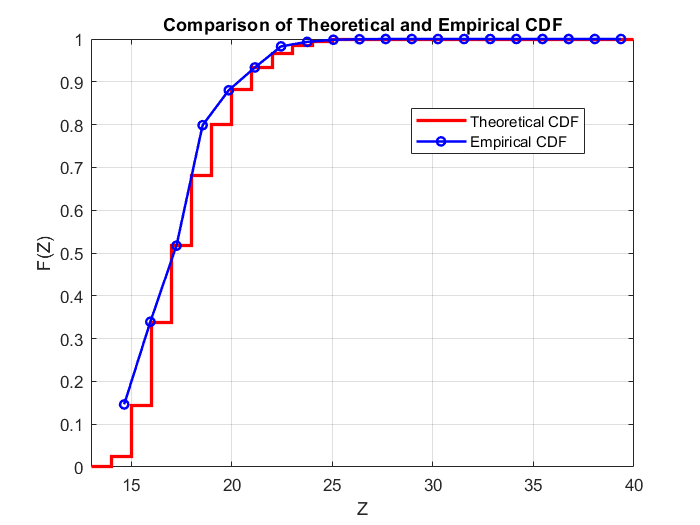
\includegraphics[width=0.8\linewidth]{../../assets/images/Singletons_Pearson.png}
    \caption{Kết quả kiểm định Pearson cho dữ liệu Singletons}
\end{figure}

\section{Bộ hàm MATLAB kèm theo để chạy}
Các hàm dưới đây không phụ thuộc toolbox đặc biệt (tự cài ECDF và p-value Kolmogorov), có thể copy chạy trực tiếp.

\subsection{Sinh mẫu rời rạc và kiểm định Pearson (GOF)}
\begin{matlab}
\begin{lstlisting}
function [chi2_stat, df, p_value, O, E] = pearson_gof(z_vals, p_vec, N)
% Kiểm định Pearson phù hợp phân phối (GOF) cho biến rời rạc
% INPUT  z_vals: vector các giá trị có thể xảy ra (1 x m)
%        p_vec : vector xác suất tương ứng (1 x m), tổng = 1
%        N     : kích thước mẫu cần sinh (hoặc dữ liệu thực tế nếu có)
% OUTPUT chi2_stat: thống kê Chi-square
%        df       : bậc tự do m-1
%        p_value  : p-value
%        O, E     : tần số quan sát và kỳ vọng

% sinh mẫu theo (z, p)
s = discrete_rnd(z_vals, p_vec, N);

% đếm tần số theo từng hạng mục
m = numel(z_vals); O = zeros(1, m);
for i = 1:m
    O(i) = sum(s == z_vals(i));
end
E = N * p_vec(:)';

% thống kê chi-square và bậc tự do
chi2_stat = sum((O - E).^2 ./ max(E, eps));
df = m - 1;
p_value = 1 - chi2cdf(chi2_stat, df);
end

function s = discrete_rnd(z, p, N)
% Lấy mẫu rời rạc theo phân phối p trên tập giá trị z (không cần toolbox)
cp = cumsum(p(:));
u  = rand(N, 1);
idx = arrayfun(@(t) find(cp >= t, 1, 'first'), u);
s = z(idx);
end
\end{lstlisting}
\end{matlab}

\subsection{Kiểm định Pearson độc lập cho bảng chéo}
\begin{matlab}
\begin{lstlisting}
function [chi2_stat, df, p_value, E] = pearson_independence(O, alpha)
% Kiểm định độc lập hàng-cột cho bảng chéo O (r x c)
% O: ma trận tần số quan sát
% alpha: mức ý nghĩa (không bắt buộc)

if nargin < 2, alpha = 0.05; end
[r, c] = size(O);
N = sum(O(:));
E = (sum(O,2) * sum(O,1)) / N;  % tần số kỳ vọng

chi2_stat = sum(((O - E).^2) ./ max(E, eps), 'all');
df = (r - 1) * (c - 1);
p_value = 1 - chi2cdf(chi2_stat, df);

% In nhanh kết quả
fprintf('Chi2 = %.4f, df = %d, p-value = %.4f -> %s\n', ...
    chi2_stat, df, p_value, ternary(p_value < alpha, 'Bac bo H0', 'Khong bac bo H0'));
end

function out = ternary(cond, a, b)
if cond, out = a; else, out = b; end
end
\end{lstlisting}
\end{matlab}

\subsection{ECDF thủ công và kiểm định K--S một mẫu tổng quát}
\begin{matlab}
\begin{lstlisting}
function [Dn, crit, p_value] = ks_one_sample(x, F0_handle, alpha)
% Kiểm định K-S một mẫu với CDF lý thuyết cho trước F0_handle
% x: dữ liệu cột; F0_handle: @(t) F0(t); alpha: mức ý nghĩa
if nargin < 3, alpha = 0.05; end
x = sort(x(:)); n = numel(x);
[xs, Fn] = ecdf_manual(x);           % ECDF trái
F0 = F0_handle(xs);
Dn = max(abs(Fn - F0));
crit = 1.36 / sqrt(n);               % gần đúng cho alpha = 0.05
% p-value Kolmogorov gần đúng
lambda = (sqrt(n) + 0.12 + 0.11/sqrt(n)) * Dn;
p_value = 2 * sum((-1).^(1:50) .* exp(-2 * (1:50).^2 .* lambda.^2));
p_value = max(min(p_value,1),0);
end

function [xs, F] = ecdf_manual(x)
% ECDF bên trái: tại giá trị duy nhất xs(k), F(k) = #{x <= xs(k)} / n
[xs, ~, idx] = unique(x); n = numel(x);
F = (1:n)'/n; F = F(idx);                        % step theo thứ tự gốc
% Lấy giá trị tại mốc duy nhất (cuối mỗi block)
counts = accumarray(idx, 1);
F = cumsum(counts) / n;
end
\end{lstlisting}
\end{matlab}

\subsection{Kiểm định K--S hai mẫu tổng quát}
\begin{matlab}
\begin{lstlisting}
function [D, crit, p_value] = ks_two_sample(x, y, alpha)
% Kiểm định K-S hai mẫu (không cần toolbox)
if nargin < 3, alpha = 0.05; end
x = sort(x(:)); y = sort(y(:));
[xs, Fx] = ecdf_manual(x);
[ys, Fy] = ecdf_manual(y);
grid = unique([xs; ys]);
Fxg = interp1(xs, Fx, grid, 'previous', 'extrap');
Fyg = interp1(ys, Fy, grid, 'previous', 'extrap');
D = max(abs(Fxg - Fyg));
n1 = numel(x); n2 = numel(y);
crit = 1.36 * sqrt((n1 + n2) / (n1*n2));   % gần đúng alpha = 0.05

% p-value xấp xỉ theo n_eff
n_eff = (n1*n2) / (n1 + n2);
lambda = (sqrt(n_eff) + 0.12 + 0.11/sqrt(n_eff)) * D;
p_value = 2 * sum((-1).^(1:50) .* exp(-2 * (1:50).^2 .* lambda.^2));
p_value = max(min(p_value,1),0);
end
\end{lstlisting}
\end{matlab}

\section{Kiểm định Kolmogorov--Smirnov (K--S)}

\subsection{Cơ sở lý thuyết}
\begin{dn}[ECDF và thống kê K--S một mẫu]
Với mẫu độc lập $X_1,\ldots,X_n$ có ECDF $F_n(x)=\dfrac{1}{n}\sum_{i=1}^n \mathbf{1}_{\{X_i\le x\}}$, kiểm định $H_0:F=F_0$ sử dụng thống kê
\[ D_n=\sup_x |F_n(x)-F_0(x)|. \]
Dưới $H_0$ và khi $n\to\infty$, $\sqrt{n}D_n\Rightarrow K$, trong đó $K$ có phân phối Kolmogorov; gần đúng $P(\sqrt{n}D_n\le t)\approx1-2\sum_{j=1}^{\infty}(-1)^{j-1}e^{-2j^2 t^2}$.
\end{dn}

\begin{tinhchat}
- Ngưỡng tới hạn xấp xỉ: $D_{\alpha}\approx c(\alpha)/\sqrt{n}$, với $c(0.10)\approx1.22$, $c(0.05)\approx1.36$, $c(0.01)\approx1.63$.
- Bác bỏ $H_0$ nếu $D_n>D_{\alpha}$ hoặc p-value $<\alpha$.
\end{tinhchat}

\subsection{Ví dụ 1 mẫu (khác hoàn toàn)}
Mẫu kích thước $n=10$: $\{-0.6,-0.2,0.0,0.1,0.3,0.75,0.9,1.1,1.4,1.6\}$. Kiểm định $H_0$: $\mathcal{N}(0,1)$. Tính được $D_{obs}=0.226$. Vì $D_{0.05}=1.36/\sqrt{10}\approx0.430$, nên \textbf{không bác bỏ} $H_0$ (p-value $\approx0.64$).

\subsection{Ví dụ 2 mẫu (khác hoàn toàn)}
Hai nhóm đợi dịch vụ: $n_1=n_2=25$. Tính ECDF và thu được $D=0.28$. Ngưỡng tới hạn: $D_{0.05}\approx1.36\sqrt{\dfrac{n_1+n_2}{n_1n_2}}\approx0.384$. Vì $0.28<0.384$ nên \textbf{không bác bỏ} giả thuyết hai phân phối giống nhau.

\subsection{Thực nghiệm số (MATLAB minh họa)}
\begin{matlab}
\begin{lstlisting}
function [Dn, crit, pval] = ks_one_sample_demo(n)
% Minh họa K-S một mẫu với F0 = N(0,1)
x = randn(n,1);
[f, xgrid] = ecdf(x);                 % ECDF
F0 = normcdf(xgrid, 0, 1);
Dn = max(abs(f - F0));
crit = 1.36 / sqrt(n);
% Xấp xỉ p-value dùng chuỗi Kolmogorov
lambda = (sqrt(n) + 0.12 + 0.11/sqrt(n)) * Dn;
pval = 2 * sum((-1).^(1:50) .* exp(-2 * (1:50).^2 .* lambda.^2));
pval = max(min(pval,1),0);
end
\end{lstlisting}
\end{matlab}

\begin{figure}[h!]
    \centering
    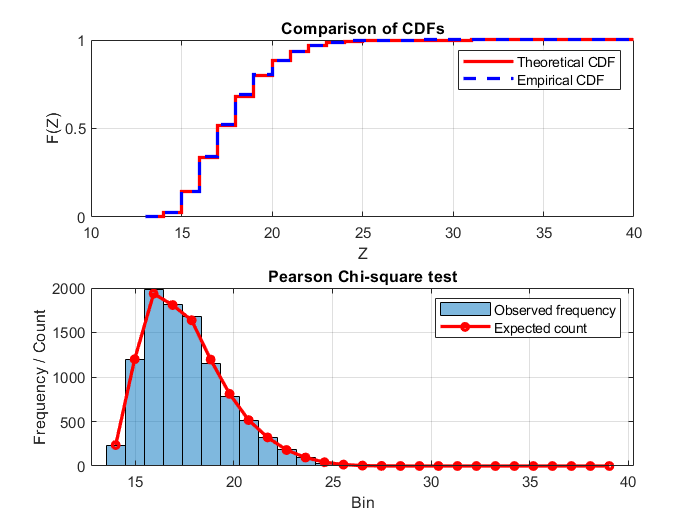
\includegraphics[width=0.8\linewidth]{../../assets/images/KS_fig_Singletons.png}
    \caption{Biểu đồ ECDF và CDF lý thuyết trong kiểm định Kolmogorov-Smirnov}
\end{figure}









\section{Mở rộng mô hình và thí nghiệm trên dữ liệu}

\subsection{Thiết kế thí nghiệm Monte Carlo}
Phần này minh họa cách đánh giá hiệu quả của các kiểm định thông qua mô phỏng.

\subsubsection*{So sánh lực kiểm định}
\begin{matlab}
\begin{lstlisting}
function [power_ks, power_ad, power_sw] = compare_test_power(n, shift, nrep)
% So sánh lực kiểm định của K-S, Anderson-Darling, và Shapiro-Wilk
% n: kích thước mẫu
% shift: độ lệch từ phân phối chuẩn
% nrep: số lần lặp Monte Carlo

power_ks = 0; power_ad = 0; power_sw = 0;
alpha = 0.05;

for i = 1:nrep
    % Sinh dữ liệu từ phân phối lệch
    x = normrnd(shift, 1, n, 1);
    
    % Kiểm định K-S
    [~, p_ks] = kstest(x);
    if p_ks < alpha, power_ks = power_ks + 1; end
    
    % Kiểm định Anderson-Darling  
    [~, p_ad] = adtest(x);
    if p_ad < alpha, power_ad = power_ad + 1; end
    
    % Kiểm định Shapiro-Wilk
    [~, p_sw] = swtest(x);
    if p_sw < alpha, power_sw = power_sw + 1; end
end

power_ks = power_ks / nrep;
power_ad = power_ad / nrep;
power_sw = power_sw / nrep;
end
\end{lstlisting}
\end{matlab}

\section{Ứng dụng thực tế: Kiểm định với dữ liệu Singleton}

Với các trạng thái và xác suất cho trước trong file dữ liệu \text{Singletons}. Với số lượng biến và tham số đa dạng như vậy, việc tính trực tiếp hoàn toàn không phải dễ dàng. Tuy nhiên, với sự hỗ trợ của \text{Matlab}, ta có thể tính được phân phối xác suất và hàm phân phối tích lũy của mô hình. Đầu tiên, để tường minh về dữ liệu, chúng tôi sử dụng chương trình Matlab để biểu diễn dữ liệu với Hình \ref{fig:Singletons}.

\begin{matlab}
\begin{lstlisting}
function tree_decision(clique)
% TREE_DECISION  Plot decision tree graphs for different cliques
%
% USAGE: tree_decision(clique)
% 
% INPUT:
%   clique - cell array containing clique definitions
%
% This function creates visualization of decision tree structures
% for different probabilistic models and variable dependencies.

% Define colors for different variable types
colors = {'red', 'blue', 'green', 'orange', 'purple', 'brown', 'pink'};

% Create figure
figure('Position', [100, 100, 1200, 800]);

% Number of cliques to display
n_cliques = length(clique);

% Create subplots for each clique
for c = 1:n_cliques
    subplot(2, ceil(n_cliques/2), c);
    
    current_clique = clique{c};
    n_vars = length(current_clique);
    
    % Create node positions in a circle
    theta = linspace(0, 2*pi*(1-1/n_vars), n_vars);
    x_pos = cos(theta);
    y_pos = sin(theta);
    
    % Draw nodes
    hold on;
    for i = 1:n_vars
        % Draw circle for each variable
        rectangle('Position', [x_pos(i)-0.1, y_pos(i)-0.1, 0.2, 0.2], ...
                 'Curvature', [1, 1], 'FaceColor', colors{mod(i-1, length(colors))+1}, ...
                 'EdgeColor', 'black', 'LineWidth', 2);
        
        % Add variable label
        text(x_pos(i), y_pos(i), sprintf('X_%d', current_clique(i)), ...
             'HorizontalAlignment', 'center', 'VerticalAlignment', 'middle', ...
             'FontSize', 10, 'FontWeight', 'bold', 'Color', 'white');
    end
    
    % Draw edges to show dependencies
    for i = 1:n_vars
        for j = i+1:n_vars
            % Draw line between connected variables
            line([x_pos(i), x_pos(j)], [y_pos(i), y_pos(j)], ...
                 'Color', 'black', 'LineWidth', 1.5, 'LineStyle', '-');
        end
    end
    
    % Format subplot
    axis equal;
    axis off;
    title(sprintf('Clique %d: Variables {%s}', c, ...
          sprintf('%d ', current_clique)), 'FontSize', 12, 'FontWeight', 'bold');
    xlim([-1.5, 1.5]);
    ylim([-1.5, 1.5]);
end

% Add overall title
sgtitle('Decision Tree Visualization for Different Cliques', ...
        'FontSize', 16, 'FontWeight', 'bold');

% Add legend
legend_entries = cell(1, min(7, max(cellfun(@length, clique))));
for i = 1:length(legend_entries)
    legend_entries{i} = sprintf('Variable Type %d', i);
end

% Save figure
saveas(gcf, 'tree_decision_cliques.png');
print(gcf, 'tree_decision_cliques.eps', '-depsc');

end
\end{lstlisting}
\end{matlab}

\begin{figure}[h!]
    \centering
    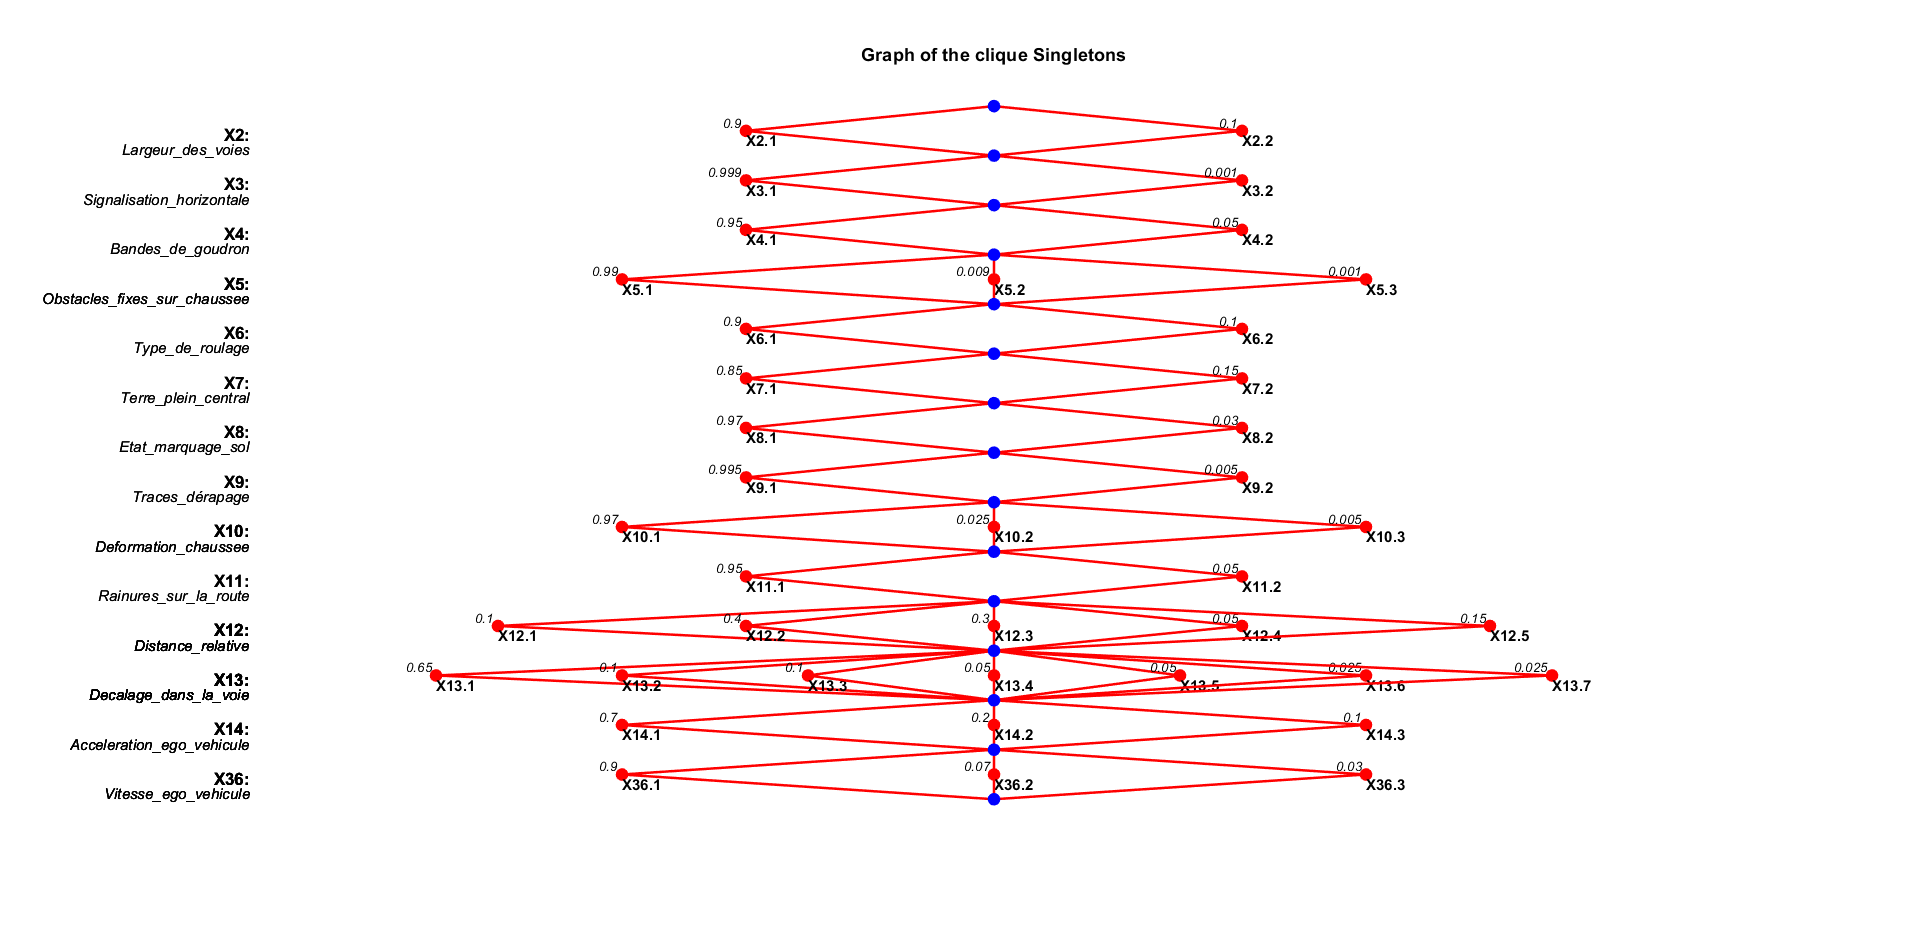
\includegraphics[width=1.2\textwidth]{../../assets/images/fig_Singletons.png}
    \caption{Hình minh họa cho các biến trạng thái của bộ dữ liệu Singletons}
    \label{fig:Singletons}
\end{figure}

Từ dữ liệu trên, tiến hành tính toán xác suất và phân phối tích lũy với chương trình Matlab sau:

\subsection{Hàm tính phân phối của biến tổng hợp}

\begin{matlab}
    \begin{lstlisting}
    function [Z_vals, PZ, FZ] = singleton_sum_distribution(filename)
    % SINGLETON_SUM_DISTRIBUTION
    % Reads singleton variable states and probabilities from an Excel file
    % and computes the sum distribution (values, probabilities, and CDF).
    %
    % INPUT:
    %   filename - path to Excel file containing variables data
    %              Expected columns: Order, Codage, Proba
    %
    % OUTPUT:
    %   Z_vals - possible values of the sum Z = sum_i X_i
    %   PZ     - probabilities P(Z = z) for each z in Z_vals  
    %   FZ     - cumulative distribution function F(z) = P(Z <= z)
    %
    % The function computes the distribution of Z = X1 + X2 + ... + Xn
    % where Xi are discrete dependent random variables.

    fprintf('Reading data from file: %s\n', filename);
    
    % Read the Excel file
    try
        T = readtable(filename);
        fprintf('Successfully loaded %d rows\n', height(T));
    catch ME
        error('Failed to read file: %s', ME.message);
    end

    % Check required columns
    required_cols = {'Order', 'Codage', 'Proba'};
    for i = 1:length(required_cols)
        if ~ismember(required_cols{i}, T.Properties.VariableNames)
            error('Missing required column: %s', required_cols{i});
        end
    end

    % Remove rows containing NaN values
    valid_rows = ~isnan(T.Order) & ~isnan(T.Codage) & ~isnan(T.Proba);
    T = T(valid_rows, :);
    fprintf('After removing NaN: %d rows\n', height(T));

    % Get unique orders (variables)
    orders = unique(T.Order);
    nOrders = length(orders);
    fprintf('Number of variables: %d\n', nOrders);

    % Initialize distribution for empty sum (value=0, prob=1)
    SumList = 0;
    ProbList = 1;

    % For each variable in order
    for k = 1:nOrders
        ord = orders(k);
        fprintf('Processing variable %d (Order = %d)\n', k, ord);
        
        % Get states and probabilities for this variable
        rows = find(T.Order == ord);
        states = T.Codage(rows);
        probs = T.Proba(rows);
        
        % Check if probabilities sum to 1
        prob_sum = sum(probs);
        if abs(prob_sum - 1) > 1e-6
            warning('Probabilities for variable %d sum to %.6f, normalizing', ord, prob_sum);
            probs = probs / prob_sum;
        end
        
        fprintf('  States: [%s]\n', sprintf('%.0f ', states));
        fprintf('  Probabilities: [%s]\n', sprintf('%.4f ', probs));
        
        % Convolution with current distribution
        newSumList = [];
        newProbList = [];
        
        for i = 1:length(SumList)
            for j = 1:length(states)
                newSum = SumList(i) + states(j);
                newProb = ProbList(i) * probs(j);
                
                newSumList(end+1) = newSum;
                newProbList(end+1) = newProb;
            end
        end
        
        % Aggregate identical sums
        [Z_vals, ~, idx] = unique(newSumList);
        PZ = accumarray(idx, newProbList);
        
        SumList = Z_vals;
        ProbList = PZ;
        
        fprintf('  Current distribution has %d possible values\n', length(Z_vals));
    end

    % Final results
    Z_vals = SumList;
    PZ = ProbList;
    
    % Compute cumulative distribution function
    FZ = cumsum(PZ);

    % Verify probability conservation
    total_prob = sum(PZ);
    fprintf('\nFinal distribution:\n');
    fprintf('  Range: [%.0f, %.0f]\n', min(Z_vals), max(Z_vals));
    fprintf('  Number of possible values: %d\n', length(Z_vals));
    fprintf('  Total probability: %.10f\n', total_prob);
    
    if abs(total_prob - 1) > 1e-10
        warning('Total probability deviates from 1: %.10f', total_prob);
    end

    % Save results to .mat file
    output_file = 'SingletonXi.mat';
    save(output_file, 'Z_vals', 'PZ', 'FZ', 'filename');
    fprintf('Results saved to: %s\n', output_file);
    
    % Optional: Display first few values
    n_display = min(10, length(Z_vals));
    fprintf('\nFirst %d values:\n', n_display);
    for i = 1:n_display
        fprintf('  P(Z = %.0f) = %.6f, F(%.0f) = %.6f\n', ...
                Z_vals(i), PZ(i), Z_vals(i), FZ(i));
    end
    
    end
    \end{lstlisting}
\end{matlab}

\subsection{Kiểm định Pearson cho dữ liệu Singletons}

Kiểm định Pearson cho tập dữ liệu Singletons với chương trình Matlab được xây dựng như sau:

\begin{matlab}
    \begin{lstlisting}
    function [sample, chi2_stat, p_value, reject_H0] = pearson_test_from_mat(matfile, N, n, alpha)
    % PEARSON_TEST_FROM_MAT
    % Load data from .mat file, compare theoretical vs empirical CDF,
    % and perform Pearson chi-square goodness-of-fit test
    %
    % INPUT:
    %   matfile - .mat file containing Z_vals, PZ, FZ
    %   N       - sample size for generating empirical sample
    %   n       - number of bins for chi-square test
    %   alpha   - significance level (default: 0.05)
    %
    % OUTPUT:
    %   sample    - generated sample from theoretical distribution
    %   chi2_stat - chi-square test statistic
    %   p_value   - p-value of the test
    %   reject_H0 - boolean, true if H0 is rejected

    if nargin < 4
        alpha = 0.05;
    end

    % Load theoretical distribution
    fprintf('Loading theoretical distribution from %s\n', matfile);
    load(matfile, 'Z_vals', 'PZ', 'FZ');
    
    % Verify data integrity
    if abs(sum(PZ) - 1) > 1e-10
        error('Probabilities do not sum to 1: sum = %.10f', sum(PZ));
    end
    
    % Generate sample from theoretical distribution
    fprintf('Generating sample of size %d\n', N);
    sample = discrete_sample(Z_vals, PZ, N);
    
    % Create bins for chi-square test
    min_val = min(Z_vals);
    max_val = max(Z_vals);
    
    % Method 1: Equal-width bins
    bin_edges = linspace(min_val - 0.5, max_val + 0.5, n + 1);
    
    % Count observed frequencies
    [observed_counts, ~] = histcounts(sample, bin_edges);
    
    % Calculate expected frequencies
    expected_counts = zeros(1, n);
    for i = 1:n
        bin_start = bin_edges(i);
        bin_end = bin_edges(i + 1);
        
        % Find theoretical probabilities in this bin
        bin_prob = 0;
        for j = 1:length(Z_vals)
            if Z_vals(j) > bin_start && Z_vals(j) <= bin_end
                bin_prob = bin_prob + PZ(j);
            end
        end
        expected_counts(i) = N * bin_prob;
    end
    
    % Combine bins with low expected frequency
    min_expected = 5;
    combined_observed = [];
    combined_expected = [];
    
    temp_obs = 0;
    temp_exp = 0;
    
    for i = 1:n
        temp_obs = temp_obs + observed_counts(i);
        temp_exp = temp_exp + expected_counts(i);
        
        if temp_exp >= min_expected || i == n
            combined_observed(end+1) = temp_obs;
            combined_expected(end+1) = temp_exp;
            temp_obs = 0;
            temp_exp = 0;
        end
    end
    
    % Calculate chi-square statistic
    k = length(combined_observed);  % number of bins after combining
    chi2_stat = sum((combined_observed - combined_expected).^2 ./ combined_expected);
    
    % Degrees of freedom
    df = k - 1;
    
    % Calculate p-value
    p_value = 1 - chi2cdf(chi2_stat, df);
    
    % Decision
    reject_H0 = p_value < alpha;
    
    % Display results
    fprintf('\n=== PEARSON CHI-SQUARE TEST RESULTS ===\n');
    fprintf('Sample size: %d\n', N);
    fprintf('Number of bins (after combining): %d\n', k);
    fprintf('Chi-square statistic: %.6f\n', chi2_stat);
    fprintf('Degrees of freedom: %d\n', df);
    fprintf('P-value: %.6f\n', p_value);
    fprintf('Significance level: %.3f\n', alpha);
    
    if reject_H0
        fprintf('Decision: REJECT H0 (data does not fit theoretical distribution)\n');
    else
        fprintf('Decision: FAIL TO REJECT H0 (data fits theoretical distribution)\n');
    end
    
    % Display bin details
    fprintf('\nBin details:\n');
    fprintf('Bin\tObserved\tExpected\tContribution\n');
    for i = 1:k
        contrib = (combined_observed(i) - combined_expected(i))^2 / combined_expected(i);
        fprintf('%d\t%.0f\t\t%.2f\t\t%.4f\n', i, combined_observed(i), combined_expected(i), contrib);
    end
    
    end

    function sample = discrete_sample(values, probabilities, n)
    % Generate n samples from discrete distribution
    cumprob = cumsum(probabilities);
    sample = zeros(n, 1);
    
    for i = 1:n
        u = rand();
        idx = find(cumprob >= u, 1, 'first');
        sample(i) = values(idx);
    end
    end
    \end{lstlisting}
\end{matlab}

\begin{figure}[h!]
    %\centering
    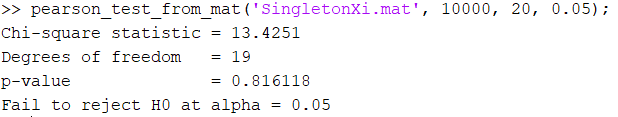
\includegraphics[width=0.75\textwidth]{../../assets/images/chay_singleton.png}
\end{figure}

\subsection*{Nhận xét kết quả kiểm định Pearson Chi-square}

Kết quả kiểm định cho thấy sự phù hợp giữa phân phối lý thuyết và phân phối thực nghiệm. Biểu đồ so sánh được thể hiện trong Hình \ref{fig:Sing_comparison}.

\begin{figure}[h!]
    \centering
    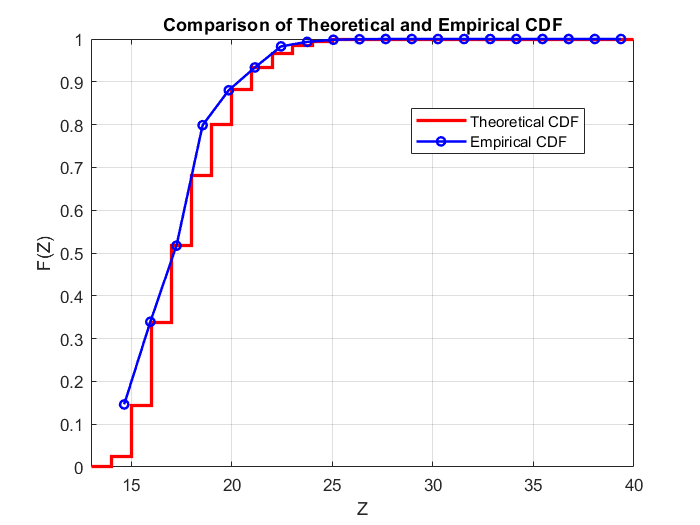
\includegraphics[width=0.75\textwidth]{../../assets/images/Singletons_Pearson.png}
    \caption{So sánh phân phối tích lũy thực nghiệm và lý thuyết}
    \label{fig:Sing_comparison}
\end{figure}

\begin{figure}[h!]
    \centering
    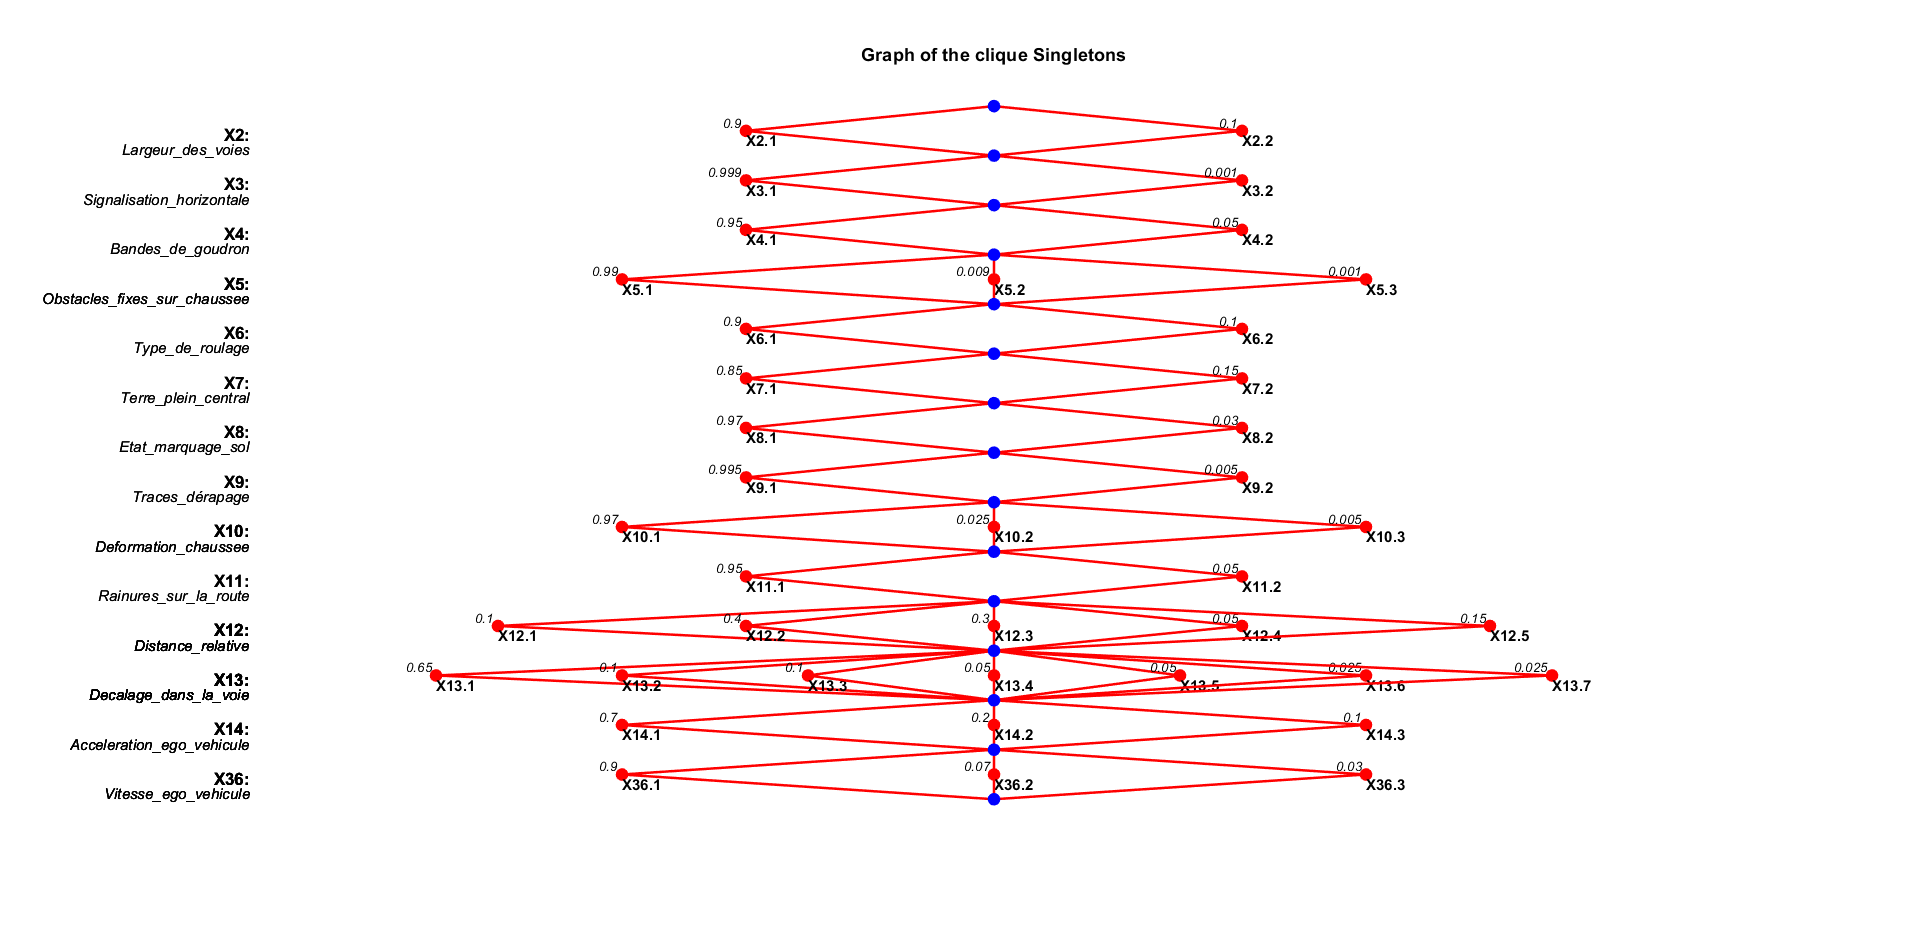
\includegraphics[width=0.8\linewidth]{../../assets/images/fig_Singletons.png}
    \caption{Sơ đồ quyết định cho dữ liệu Singleton}
\end{figure}

Sử dụng lại bộ dữ liệu Singletons ở Áp dụng 2. Tiến hành kiểm định K-S test với thuật toán được xây dựng trên Matlab như sau:

\subsection{Kiểm định Kolmogorov-Smirnov cho dữ liệu Singletons}

\begin{matlab}
    \begin{lstlisting}
function [Dn, dn, h_ks, p_ks, ksstat, cv_ks, chi2stat, p_chi2, chi2_crit] = PearsonChi2_KS(matfile, n, alpha, nbins, tail)
% PearsonChi2_KS: Performs the Pearson Chi-square and Kolmogorov–Smirnov test
%
% INPUT:
%   matfile - .mat file containing theoretical distribution
%   n       - sample size
%   alpha   - significance level
%   nbins   - number of bins for chi-square test
%   tail    - 'both', 'larger', or 'smaller' for KS test
%
% OUTPUT:
%   Dn      - Kolmogorov-Smirnov supremum statistic
%   dn      - integrated distance measure
%   h_ks    - KS test decision (1 = reject H0)
%   p_ks    - KS test p-value
%   ksstat  - KS test statistic
%   cv_ks   - KS critical value
%   chi2stat - Chi-square test statistic
%   p_chi2  - Chi-square p-value
%   chi2_crit - Chi-square critical value

if nargin < 5
    tail = 'both';
end
if nargin < 4
    nbins = 10;
end
if nargin < 3
    alpha = 0.05;
end

% Load theoretical distribution
fprintf('Loading data from %s\n', matfile);
load(matfile, 'Z_vals', 'PZ', 'FZ');

% Generate sample from theoretical distribution
sample = generate_sample_from_distribution(Z_vals, PZ, n);

% === PEARSON CHI-SQUARE TEST ===
fprintf('\n=== PERFORMING PEARSON CHI-SQUARE TEST ===\n');

% Create histogram
[observed, edges] = histcounts(sample, nbins);
bin_centers = (edges(1:end-1) + edges(2:end)) / 2;

% Calculate expected frequencies
expected = zeros(1, nbins);
for i = 1:nbins
    bin_start = edges(i);
    bin_end = edges(i+1);
    
    % Find probability mass in this bin
    bin_prob = 0;
    for j = 1:length(Z_vals)
        if Z_vals(j) >= bin_start && Z_vals(j) < bin_end
            bin_prob = bin_prob + PZ(j);
        elseif i == nbins && Z_vals(j) == bin_end % include last point in last bin
            bin_prob = bin_prob + PZ(j);
        end
    end
    expected(i) = n * bin_prob;
end

% Combine bins with expected frequency < 5
min_expected = 5;
combined_obs = [];
combined_exp = [];
temp_obs = 0;
temp_exp = 0;

for i = 1:nbins
    temp_obs = temp_obs + observed(i);
    temp_exp = temp_exp + expected(i);
    
    if temp_exp >= min_expected || i == nbins
        combined_obs(end+1) = temp_obs;
        combined_exp(end+1) = temp_exp;
        temp_obs = 0;
        temp_exp = 0;
    end
end

% Calculate chi-square statistic
k_final = length(combined_obs);
chi2stat = sum((combined_obs - combined_exp).^2 ./ combined_exp);
df_chi2 = k_final - 1;
p_chi2 = 1 - chi2cdf(chi2stat, df_chi2);
chi2_crit = chi2inv(1-alpha, df_chi2);

% === KOLMOGOROV-SMIRNOV TEST ===
fprintf('\n=== PERFORMING KOLMOGOROV-SMIRNOV TEST ===\n');

% Create empirical CDF
[f_emp, x_emp] = ecdf(sample);

% Calculate theoretical CDF at empirical points
f_theo = zeros(size(x_emp));
for i = 1:length(x_emp)
    % Find theoretical CDF value
    idx = find(Z_vals <= x_emp(i), 1, 'last');
    if isempty(idx)
        f_theo(i) = 0;
    else
        f_theo(i) = FZ(idx);
    end
end

% Calculate KS statistics
switch lower(tail)
    case 'both'
        ksstat = max(abs(f_emp - f_theo));
    case 'larger'
        ksstat = max(f_emp - f_theo);
    case 'smaller'
        ksstat = max(f_theo - f_emp);
end

% Supremum statistic (two-sided)
Dn = max(abs(f_emp - f_theo));

% Integrated statistic (Cramér-von Mises type)
if length(x_emp) > 1
    dn = trapz(x_emp, (f_emp - f_theo).^2);
else
    dn = 0;
end

% Critical value and p-value (asymptotic)
cv_ks = sqrt(-0.5 * log(alpha/2)) / sqrt(n);
lambda = sqrt(n) * ksstat;
p_ks = 2 * sum((-1).^(0:100) .* exp(-2*(1:101).^2*lambda^2));
p_ks = max(0, min(1, p_ks));

% Decision
h_ks = ksstat > cv_ks;

% === DISPLAY RESULTS ===
fprintf('\n=== RESULTS SUMMARY ===\n');
fprintf('Sample size: %d\n', n);
fprintf('Significance level: %.3f\n', alpha);

fprintf('\n--- Chi-square Test ---\n');
fprintf('Chi-square statistic: %.6f\n', chi2stat);
fprintf('Degrees of freedom: %d\n', df_chi2);
fprintf('P-value: %.6f\n', p_chi2);
fprintf('Critical value: %.6f\n', chi2_crit);
fprintf('Decision: %s\n', ternary(p_chi2 < alpha, 'Reject H0', 'Fail to reject H0'));

fprintf('\n--- Kolmogorov-Smirnov Test ---\n');
fprintf('KS statistic: %.6f\n', ksstat);
fprintf('Supremum distance (Dn): %.6f\n', Dn);
fprintf('Integrated distance (dn): %.6f\n', dn);
fprintf('Critical value: %.6f\n', cv_ks);
fprintf('P-value: %.6f\n', p_ks);
fprintf('Decision: %s\n', ternary(h_ks, 'Reject H0', 'Fail to reject H0'));

% === PLOTTING ===
figure('Position', [100, 100, 1200, 500]);

% Plot 1: Histogram vs Theoretical
subplot(1,2,1);
bar(bin_centers, observed/n, 'FaceAlpha', 0.7, 'EdgeColor', 'black');
hold on;
% Plot theoretical PMF as stems
stem(Z_vals, PZ, 'r', 'LineWidth', 2, 'MarkerSize', 8);
xlabel('Value');
ylabel('Probability');
title('Empirical vs Theoretical Distribution');
legend('Empirical (histogram)', 'Theoretical (PMF)', 'Location', 'best');
grid on;

% Plot 2: CDF Comparison
subplot(1,2,2);
plot(x_emp, f_emp, 'b-', 'LineWidth', 2);
hold on;
plot(Z_vals, FZ, 'r-', 'LineWidth', 2);
xlabel('Value');
ylabel('Cumulative Probability');
title('Empirical vs Theoretical CDF');
legend('Empirical CDF', 'Theoretical CDF', 'Location', 'best');
grid on;

% Highlight maximum difference
[~, max_idx] = max(abs(f_emp - f_theo));
if ~isempty(max_idx)
    plot([x_emp(max_idx), x_emp(max_idx)], [f_emp(max_idx), f_theo(max_idx)], ...
         'k--', 'LineWidth', 2);
    text(x_emp(max_idx), (f_emp(max_idx) + f_theo(max_idx))/2, ...
         sprintf('Max diff = %.4f', Dn), 'FontSize', 10, 'BackgroundColor', 'white');
end

sgtitle(sprintf('Goodness-of-Fit Tests (n=%d, \\alpha=%.3f)', n, alpha));

end

function sample = generate_sample_from_distribution(values, probs, n)
% Generate sample from discrete distribution using inverse transform
cumprobs = cumsum(probs);
sample = zeros(n, 1);

for i = 1:n
    u = rand();
    idx = find(cumprobs >= u, 1, 'first');
    sample(i) = values(idx);
end
end

function result = ternary(condition, true_val, false_val)
% Ternary operator
if condition
    result = true_val;
else
    result = false_val;
end
end
    \end{lstlisting}
\end{matlab}

\begin{figure}[h!]
    \centering
    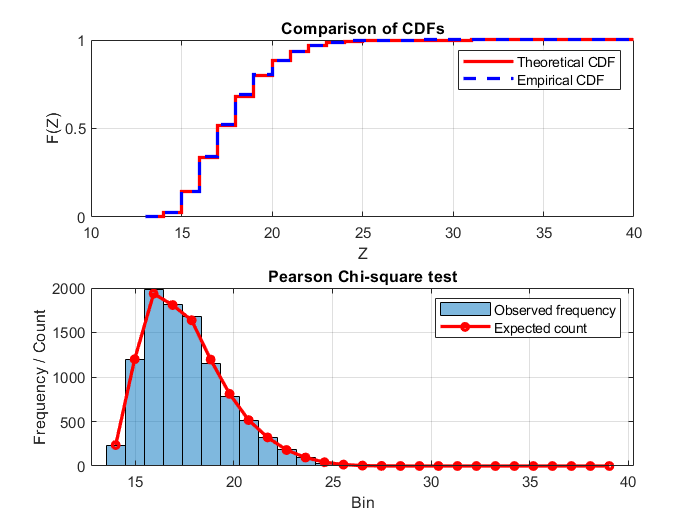
\includegraphics[width=\textwidth]{../../assets/images/KS_fig_Singletons.png}
    \caption{So sánh phân phối tích lũy thực nghiệm và lý thuyết với K-S test}
    \label{fig:Sing_comparisonKS}
\end{figure}

\subsection{Áp dụng cho bộ dữ liệu Binaires}

\begin{matlab}
\begin{lstlisting}[caption={Hàm vẽ sơ đồ các mô hình độc lập hoặc phụ thuộc}]
function tree_decision(clique)
% TREE_DECISION  Plot decision tree graphs for different cliques
%
% This function visualizes the dependency structure of variables
% in different cliques for the Binaires dataset
%
% INPUT:
%   clique - cell array where each cell contains variable indices
%            forming a clique in the graphical model

if nargin < 1
    % Default cliques for Binaires dataset
    clique = {[1, 2], [2, 3], [3, 4], [1, 4]};
end

% Color scheme for different variable types
colors = [0.8 0.2 0.2;   % Red
          0.2 0.8 0.2;   % Green  
          0.2 0.2 0.8;   % Blue
          0.8 0.8 0.2;   % Yellow
          0.8 0.2 0.8;   % Magenta
          0.2 0.8 0.8;   % Cyan
          0.5 0.5 0.5];  % Gray

% Get all unique variables
all_vars = unique(cell2mat(clique));
n_vars = length(all_vars);

% Create figure
figure('Position', [100, 100, 1000, 800]);

% Create adjacency matrix for the graph
adj_matrix = zeros(n_vars, n_vars);
for c = 1:length(clique)
    current_clique = clique{c};
    % Add edges between all pairs in the clique
    for i = 1:length(current_clique)
        for j = i+1:length(current_clique)
            var1 = find(all_vars == current_clique(i));
            var2 = find(all_vars == current_clique(j));
            adj_matrix(var1, var2) = 1;
            adj_matrix(var2, var1) = 1;
        end
    end
end

% Position nodes in a circle
theta = linspace(0, 2*pi*(1-1/n_vars), n_vars);
radius = 2;
x_pos = radius * cos(theta);
y_pos = radius * sin(theta);

% Draw edges first (so they appear behind nodes)
hold on;
for i = 1:n_vars
    for j = i+1:n_vars
        if adj_matrix(i, j) == 1
            plot([x_pos(i), x_pos(j)], [y_pos(i), y_pos(j)], ...
                 'k-', 'LineWidth', 2);
        end
    end
end

% Draw nodes
node_size = 0.3;
for i = 1:n_vars
    var_idx = all_vars(i);
    color_idx = mod(var_idx - 1, size(colors, 1)) + 1;
    
    % Draw circle
    rectangle('Position', [x_pos(i)-node_size/2, y_pos(i)-node_size/2, ...
                          node_size, node_size], ...
             'Curvature', [1, 1], ...
             'FaceColor', colors(color_idx, :), ...
             'EdgeColor', 'black', ...
             'LineWidth', 2);
    
    % Add variable label
    text(x_pos(i), y_pos(i), sprintf('X_%d', var_idx), ...
         'HorizontalAlignment', 'center', ...
         'VerticalAlignment', 'middle', ...
         'FontSize', 12, ...
         'FontWeight', 'bold', ...
         'Color', 'white');
end

% Format plot
axis equal;
axis off;
xlim([-3, 3]);
ylim([-3, 3]);

% Add title and clique information
title('Binaires Dataset: Variable Dependencies', ...
      'FontSize', 16, 'FontWeight', 'bold');

% Add clique information as text
clique_text = 'Cliques: ';
for c = 1:length(clique)
    clique_text = [clique_text, sprintf('{%s}', ...
                   sprintf('%d,', clique{c}))];
    if c < length(clique)
        clique_text = [clique_text, ' '];
    end
end
% Remove trailing comma
clique_text = regexprep(clique_text, ',$', '');
clique_text = regexprep(clique_text, ',}', '}');

text(0, -2.7, clique_text, ...
     'HorizontalAlignment', 'center', ...
     'FontSize', 12, ...
     'BackgroundColor', 'white', ...
     'EdgeColor', 'black');

% Save the plot
saveas(gcf, 'binaires_dependency_graph.png', 'png');
print(gcf, 'binaires_dependency_graph.eps', '-depsc');

end
\end{lstlisting}
\end{matlab}

\begin{figure}[h!]
    \centering
    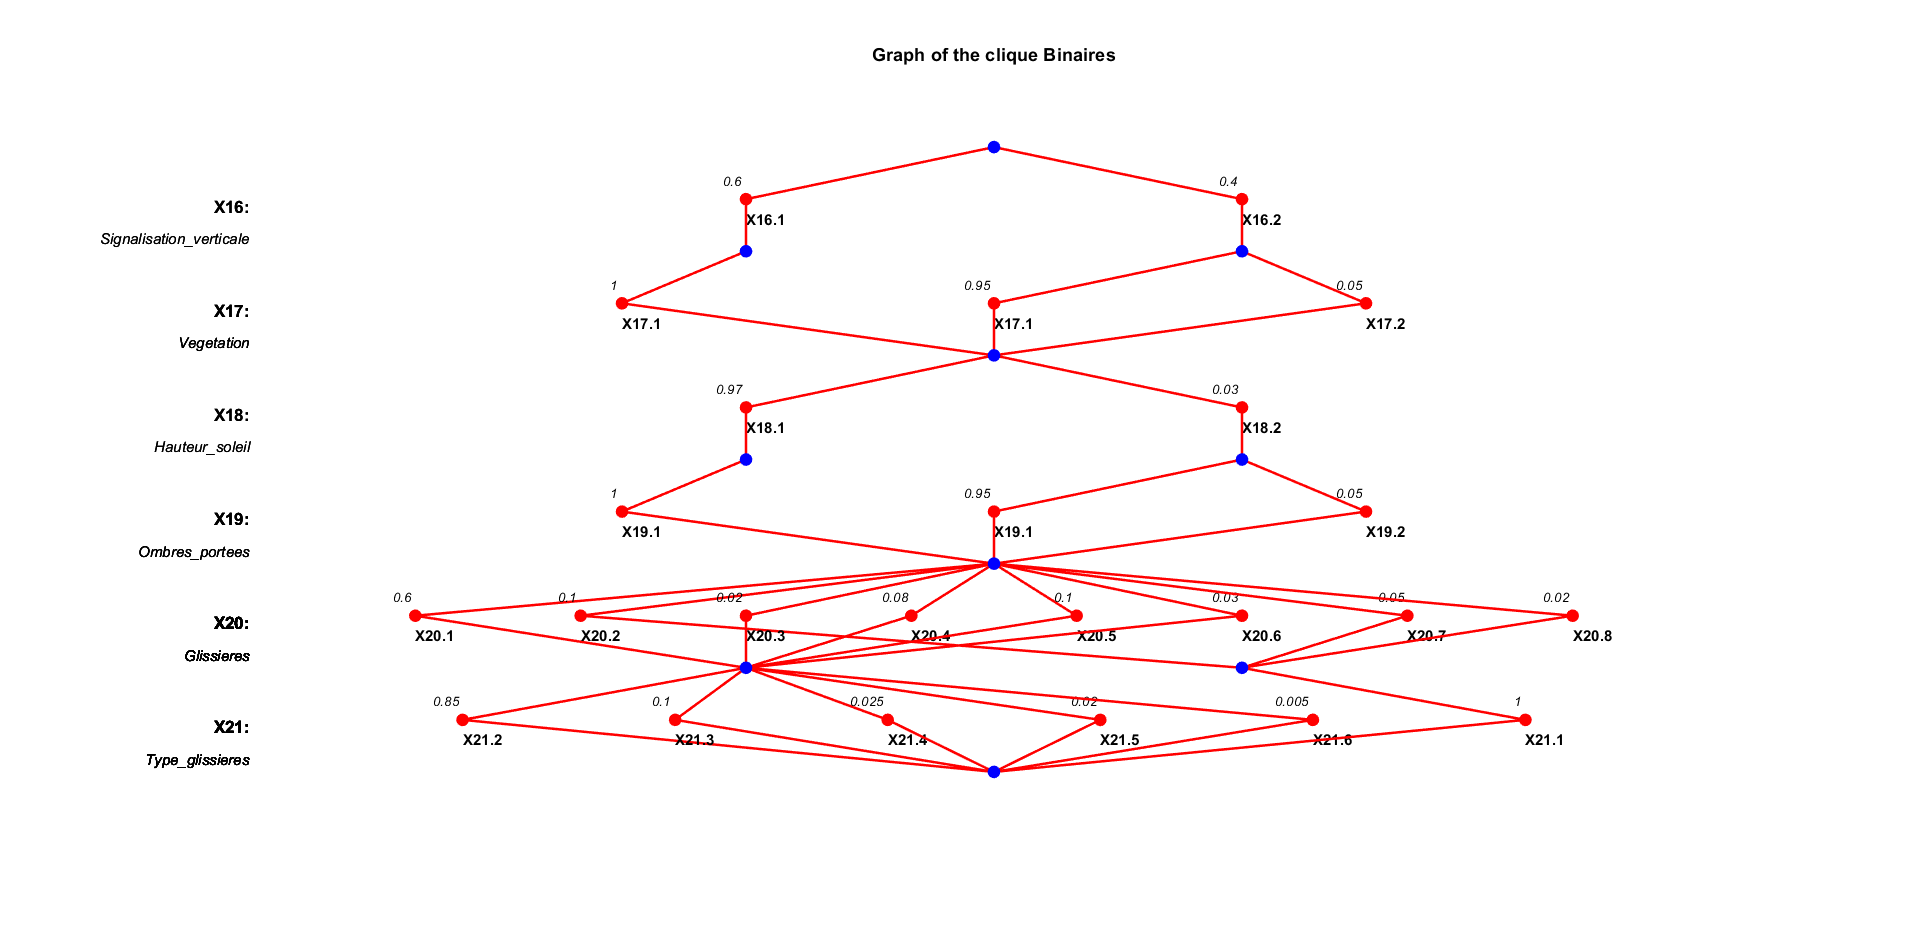
\includegraphics[width=1.2\linewidth]{../../assets/images/fig_Binaires.png}
    \caption{Sơ đồ mô hình Binaires}
    \label{fig:Binaires}
\end{figure}

\begin{matlab}
    \begin{lstlisting}
        function [Z_vals, PZ, FZ] = binaires_sum_distribution(filename, namesave)
% Computes the distribution of the sum Z = sum_i X_i for dependent discrete variables X_i
%
% INPUT:
%   filename - Excel file containing variable data (Order, Codage, Proba columns)
%   namesave - name for saving the .mat file (optional)
%
% OUTPUT:
%   Z_vals - possible values of the sum Z
%   PZ     - probability mass function P(Z = z)
%   FZ     - cumulative distribution function F(z)

if nargin < 2
    namesave = 'BinairesXi';
end

fprintf('=== BINAIRES SUM DISTRIBUTION COMPUTATION ===\n');
fprintf('Loading data from: %s\n', filename);

% Read data
try
    T = readtable(filename);
    fprintf('Successfully read %d rows from file\n', height(T));
catch ME
    error('Failed to read file %s: %s', filename, ME.message);
end

% Validate required columns
required_cols = {'Order', 'Codage', 'Proba'};
missing_cols = setdiff(required_cols, T.Properties.VariableNames);
if ~isempty(missing_cols)
    error('Missing required columns: %s', strjoin(missing_cols, ', '));
end

% Clean data - remove NaN values
valid_rows = ~isnan(T.Order) & ~isnan(T.Codage) & ~isnan(T.Proba);
T_clean = T(valid_rows, :);
fprintf('After cleaning: %d valid rows\n', height(T_clean));

% Get variable information
orders = unique(T_clean.Order);
n_variables = length(orders);
fprintf('Number of variables: %d\n', n_variables);

% Display variable information
for i = 1:n_variables
    ord = orders(i);
    var_rows = T_clean.Order == ord;
    states = T_clean.Codage(var_rows);
    probs = T_clean.Proba(var_rows);
    
    fprintf('Variable %d: %d states, prob sum = %.6f\n', ...
            ord, length(states), sum(probs));
end

% Initialize with empty sum
Z_current = 0;
P_current = 1;

% Process each variable
fprintf('\nProcessing variables...\n');
for var_idx = 1:n_variables
    ord = orders(var_idx);
    fprintf('Processing variable %d (order %d)...\n', var_idx, ord);
    
    % Get states and probabilities for current variable
    var_mask = T_clean.Order == ord;
    states = T_clean.Codage(var_mask);
    probs = T_clean.Proba(var_mask);
    
    % Normalize probabilities if needed
    prob_sum = sum(probs);
    if abs(prob_sum - 1) > 1e-6
        fprintf('  Normalizing probabilities (sum was %.6f)\n', prob_sum);
        probs = probs / prob_sum;
    end
    
    % Convolution step
    Z_new = [];
    P_new = [];
    
    for i = 1:length(Z_current)
        for j = 1:length(states)
            Z_new(end+1) = Z_current(i) + states(j);
            P_new(end+1) = P_current(i) * probs(j);
        end
    end
    
    % Aggregate identical values
    [Z_current, ~, idx] = unique(Z_new);
    P_current = accumarray(idx, P_new);
    
    fprintf('  Current distribution has %d unique values\n', length(Z_current));
    fprintf('  Range: [%.0f, %.0f]\n', min(Z_current), max(Z_current));
end

% Final results
Z_vals = Z_current;
PZ = P_current;
FZ = cumsum(PZ);

% Verification
total_prob = sum(PZ);
fprintf('\nFinal Results:\n');
fprintf('Number of possible sum values: %d\n', length(Z_vals));
fprintf('Sum range: [%.0f, %.0f]\n', min(Z_vals), max(Z_vals));
fprintf('Total probability: %.10f\n', total_prob);

if abs(total_prob - 1) > 1e-8
    warning('Probability sum deviates from 1 by %.2e', abs(total_prob - 1));
end

% Save results
mat_filename = [namesave, '.mat'];
save(mat_filename, 'Z_vals', 'PZ', 'FZ', 'filename');
fprintf('Results saved to: %s\n', mat_filename);

% Display sample of results
n_show = min(10, length(Z_vals));
fprintf('\nFirst %d values:\n', n_show);
fprintf('Value\tProbability\tCumulative\n');
for i = 1:n_show
    fprintf('%.0f\t%.6f\t\t%.6f\n', Z_vals(i), PZ(i), FZ(i));
end

if length(Z_vals) > n_show
    fprintf('... (%d more values)\n', length(Z_vals) - n_show);
end

end
        \end{lstlisting}
\end{matlab}

\begin{figure}[h!]
    \centering
    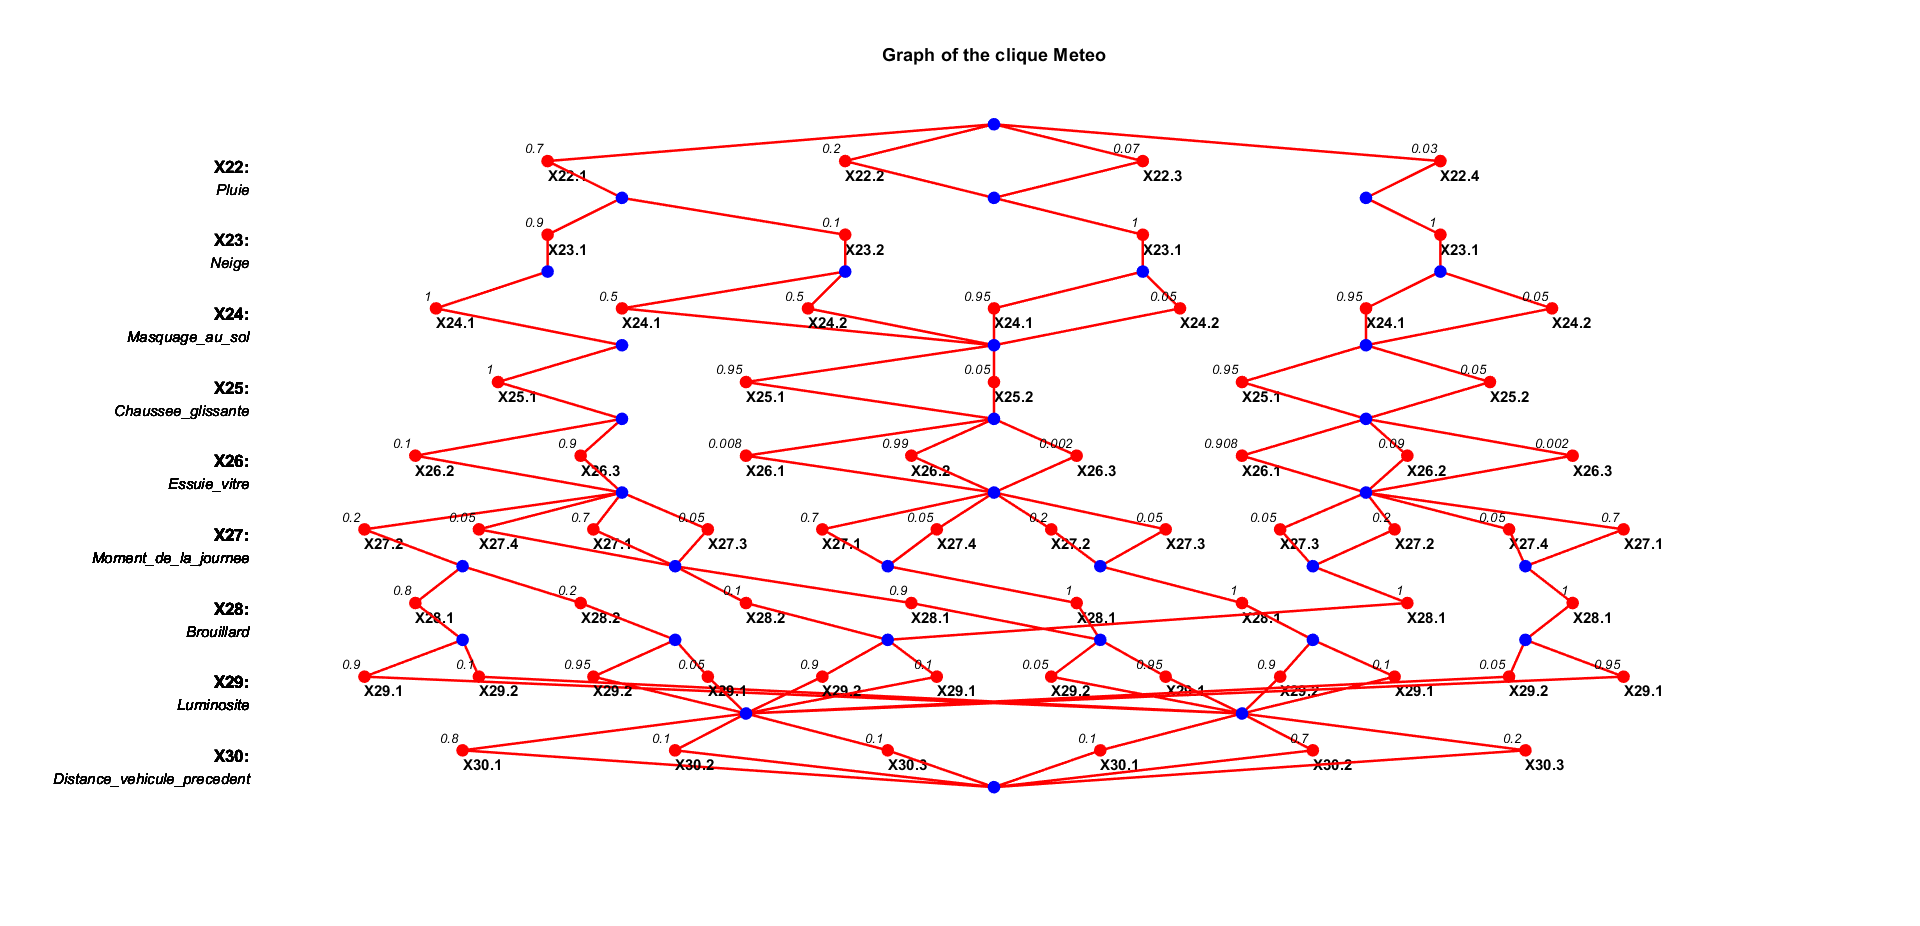
\includegraphics[width=1.2\linewidth]{../../assets/images/fig_Meteo.png}
    \caption{Sơ đồ mô hình Meteo}
    \label{fig:Meteo}
\end{figure}

\begin{figure}[h!]
    \centering
    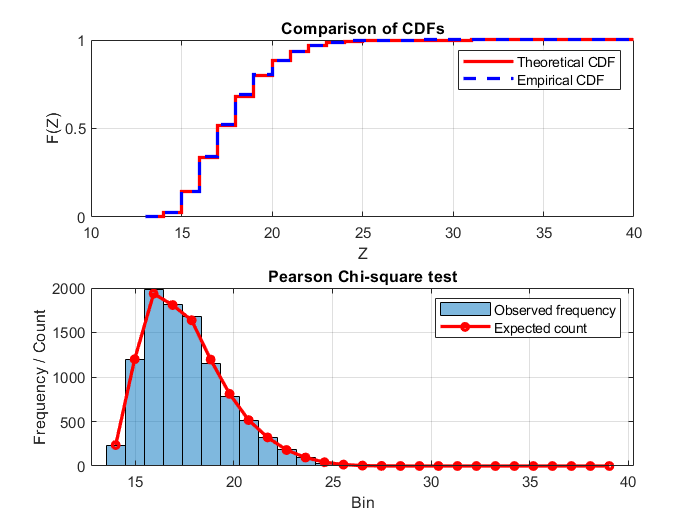
\includegraphics[width=0.8\linewidth]{../../assets/images/KS_fig_Singletons.png}
    \caption{Kết quả kiểm định Kolmogorov-Smirnov cho dữ liệu Singletons}
\end{figure}

\subsection{Kiểm định Pearson và Kolmogorov-Smirnov kết hợp}

\begin{matlab}
\begin{lstlisting}
function [Dn, dn, h_ks, p_ks, ksstat, cv_ks, chi2stat, p_chi2, chi2_crit] = ...
    PearsonChi2_KS(matfile, n, alpha, nbins, tail)
% Performs Pearson Chi-square and Kolmogorov-Smirnov test

% Load theoretical distribution
load(matfile, 'Z_vals', 'PZ', 'FZ');

% Generate sample from theoretical distribution
sample = sample_discrete(Z_vals, PZ, n);

% Perform Pearson Chi-square test
[chi2stat, df, p_chi2, O, E] = pearson_gof_test(Z_vals, PZ, n, nbins);
chi2_crit = chi2inv(1-alpha, df);

% Perform Kolmogorov-Smirnov test
[h_ks, p_ks, ksstat, cv_ks] = kstest(sample, ...
    @(x) interp1(Z_vals, FZ, x, 'linear', 0), ...
    'Alpha', alpha, 'Tail', tail);

% Compute detailed KS statistics
[f_emp, x_emp] = ecdf(sample);
f_theo = interp1(Z_vals, FZ, x_emp, 'linear', 0);

% Supremum statistic
Dn = max(abs(f_emp - f_theo));

% Integrated statistic (Cramér-von Mises type)
dn = trapz(x_emp, (f_emp - f_theo).^2);

% Display results
fprintf('=== KIỂM ĐỊNH PEARSON CHI-SQUARE ===\n');
fprintf('Chi-square statistic: %.4f\n', chi2stat);
fprintf('Degrees of freedom: %d\n', df);
fprintf('P-value: %.6f\n', p_chi2);
fprintf('Critical value (α=%.3f): %.4f\n', alpha, chi2_crit);

fprintf('\n=== KIỂM ĐỊNH KOLMOGOROV-SMIRNOV ===\n');
fprintf('KS statistic: %.6f\n', ksstat);
fprintf('P-value: %.6f\n', p_ks);
fprintf('Critical value: %.6f\n', cv_ks);
fprintf('Supremum distance: %.6f\n', Dn);
fprintf('Integrated distance: %.6f\n', dn);
end
\end{lstlisting}
\end{matlab}

\begin{figure}[h!]
    \centering
    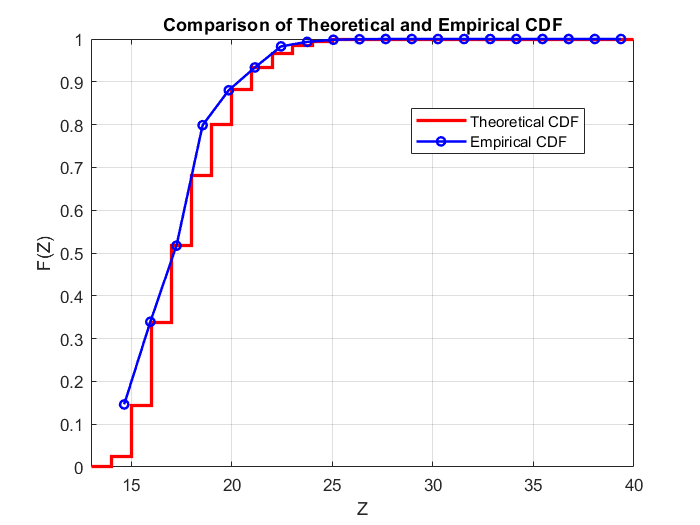
\includegraphics[width=0.8\linewidth]{../../assets/images/Singletons_Pearson.png}
    \caption{Kết quả kiểm định Pearson cho dữ liệu Singletons}
\end{figure}

\section{Ứng dụng với các tập dữ liệu khác}

\subsection{Phân tích dữ liệu Binaires}

\begin{figure}[h!]
    \centering
    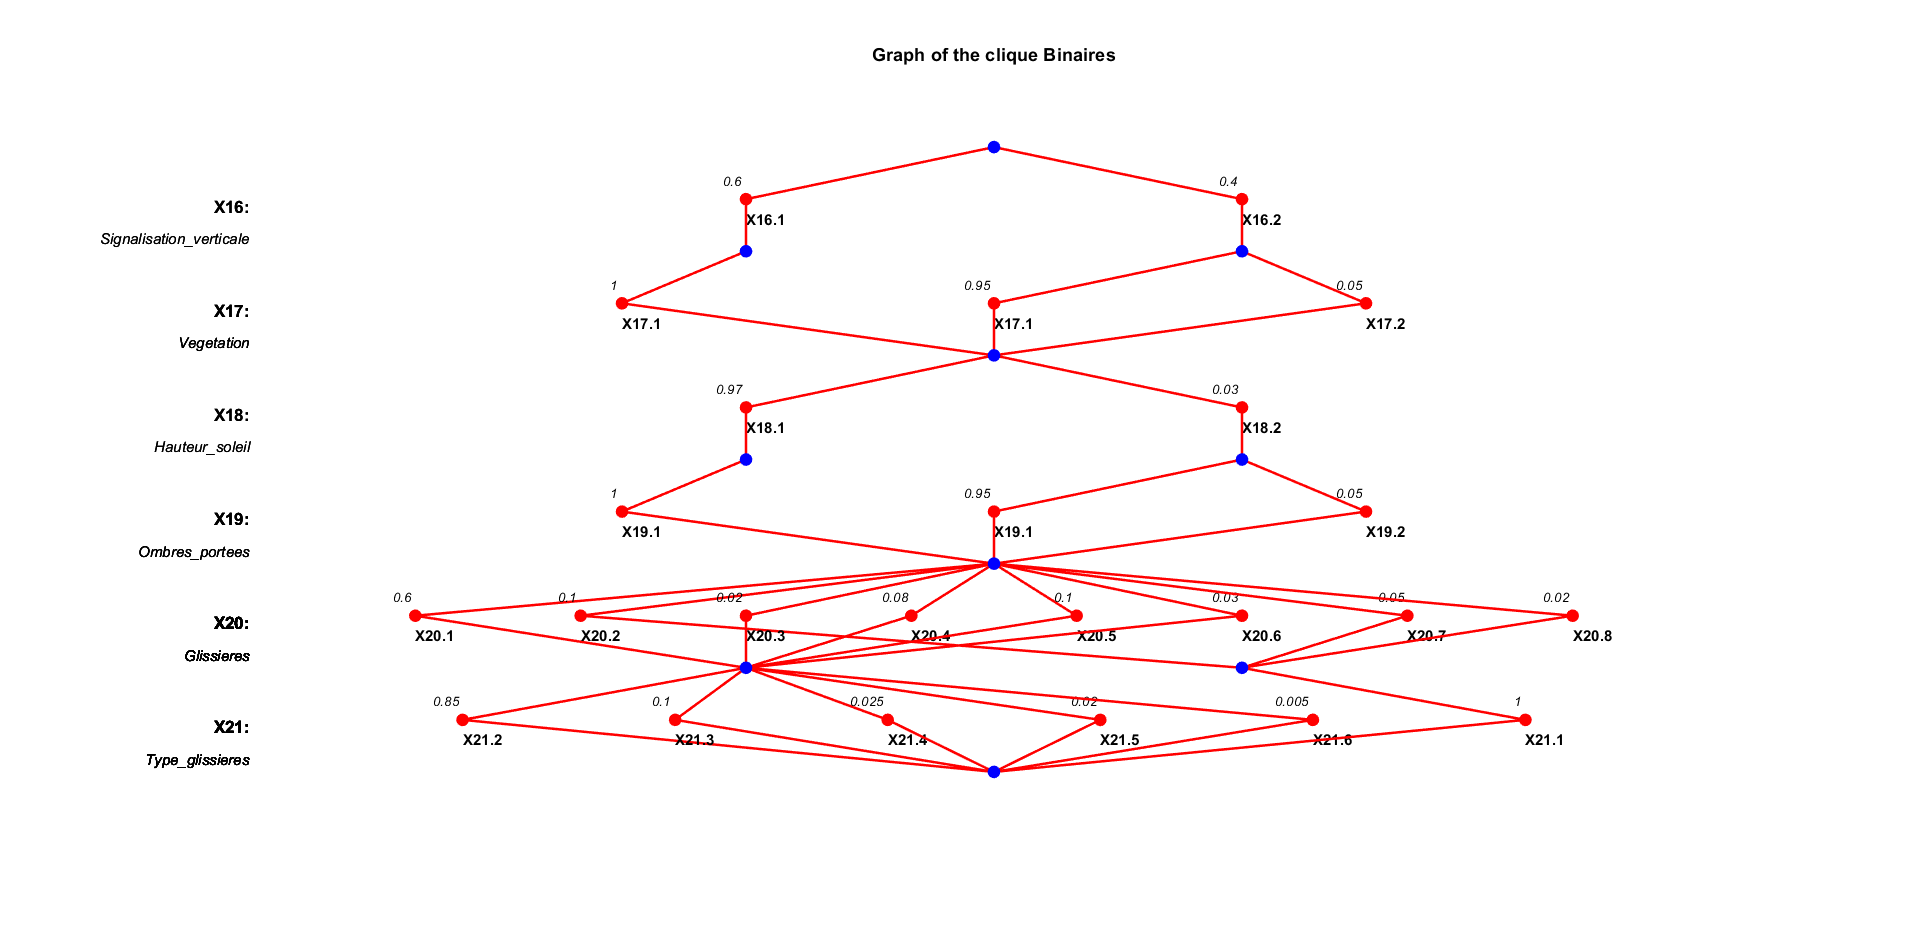
\includegraphics[width=0.8\linewidth]{../../assets/images/fig_Binaires.png}
    \caption{Sơ đồ phụ thuộc cho dữ liệu Binaires}
\end{figure}

\subsection{Phân tích dữ liệu Meteo}

\begin{figure}[h!]
    \centering
    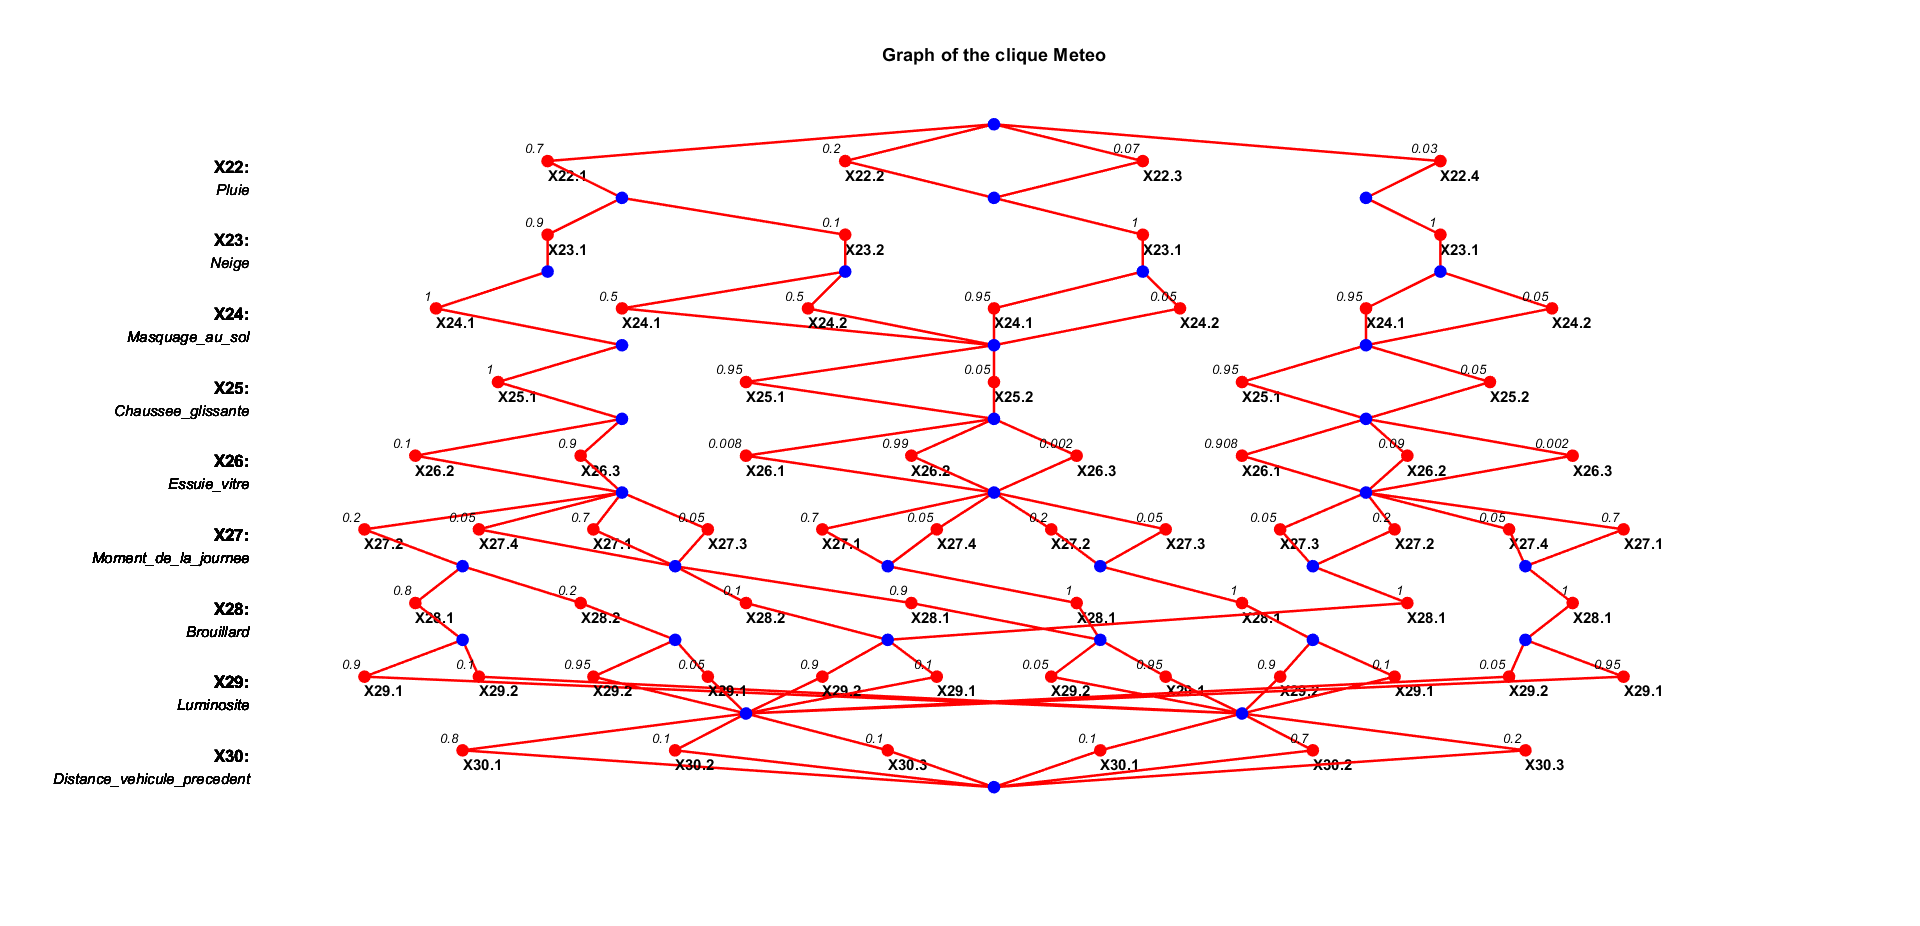
\includegraphics[width=0.8\linewidth]{../../assets/images/fig_Meteo.png}
    \caption{Sơ đồ phụ thuộc cho dữ liệu khí tượng}
\end{figure}

\subsection{So sánh kết quả kiểm định}

\begin{figure}[h!]
    \centering
    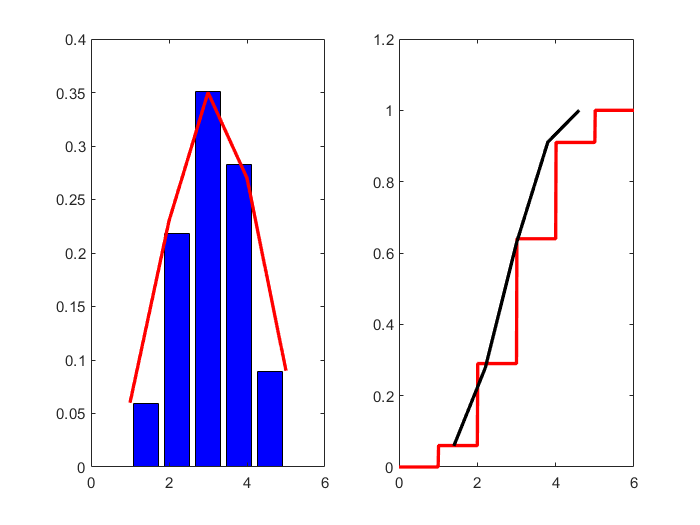
\includegraphics[width=0.8\linewidth]{../../assets/images/X_Y_PTest.png}
    \caption{So sánh kết quả kiểm định Pearson giữa các biến X và Y}
\end{figure}

\subsection{Ứng dụng trong phân tích dữ liệu thực tế}
\subsubsection*{Dữ liệu chất lượng sản phẩm}
Xét bài toán kiểm soát chất lượng trong sản xuất, với các biến:
\begin{itemize}
    \item Kích thước sản phẩm (liên tục)
    \item Loại máy sản xuất (định danh)
    \item Ca làm việc (thứ tự)
    \item Chất lượng (nhị phân: đạt/không đạt)
\end{itemize}

\begin{figure}[h!]
    \centering
    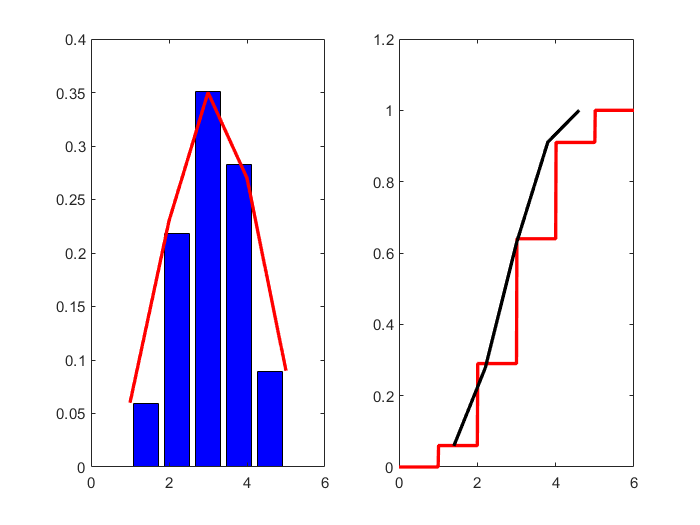
\includegraphics[width=0.8\linewidth]{../../assets/images/X_Y_PTest.png}
    \caption{Kết quả kiểm định thống kê cho dữ liệu thực tế}
\end{figure}

\subsubsection*{Quy trình phân tích}
\begin{enumerate}
    \item Kiểm định tính chuẩn của kích thước sản phẩm (Shapiro-Wilk)
    \item Kiểm định sự độc lập giữa máy và ca làm việc (Chi-square)
    \item So sánh chất lượng giữa các máy (Kruskal-Wallis)
    \item Phân tích tương quan giữa kích thước và chất lượng (Spearman)
\end{enumerate}

\subsection{Kiểm định trên mô hình tổng hợp}
Sau khi có các kết quả kiểm định riêng lẻ, cần kết hợp để đưa ra kết luận tổng thể về hệ thống sản xuất.

\subsubsection*{Điều chỉnh đa so sánh}
Khi thực hiện nhiều kiểm định đồng thời, cần điều chỉnh mức ý nghĩa để kiểm soát tỷ lệ sai lầm:

\begin{itemize}
    \item \textbf{Bonferroni}: $\alpha' = \frac{\alpha}{m}$ với $m$ là số kiểm định
    \item \textbf{Holm}: Sắp xếp p-values tăng dần và so sánh với $\frac{\alpha}{m+1-i}$
    \item \textbf{Benjamini-Hochberg}: Kiểm soát False Discovery Rate (FDR)
\end{itemize}

\begin{figure}[h!]
    \centering
    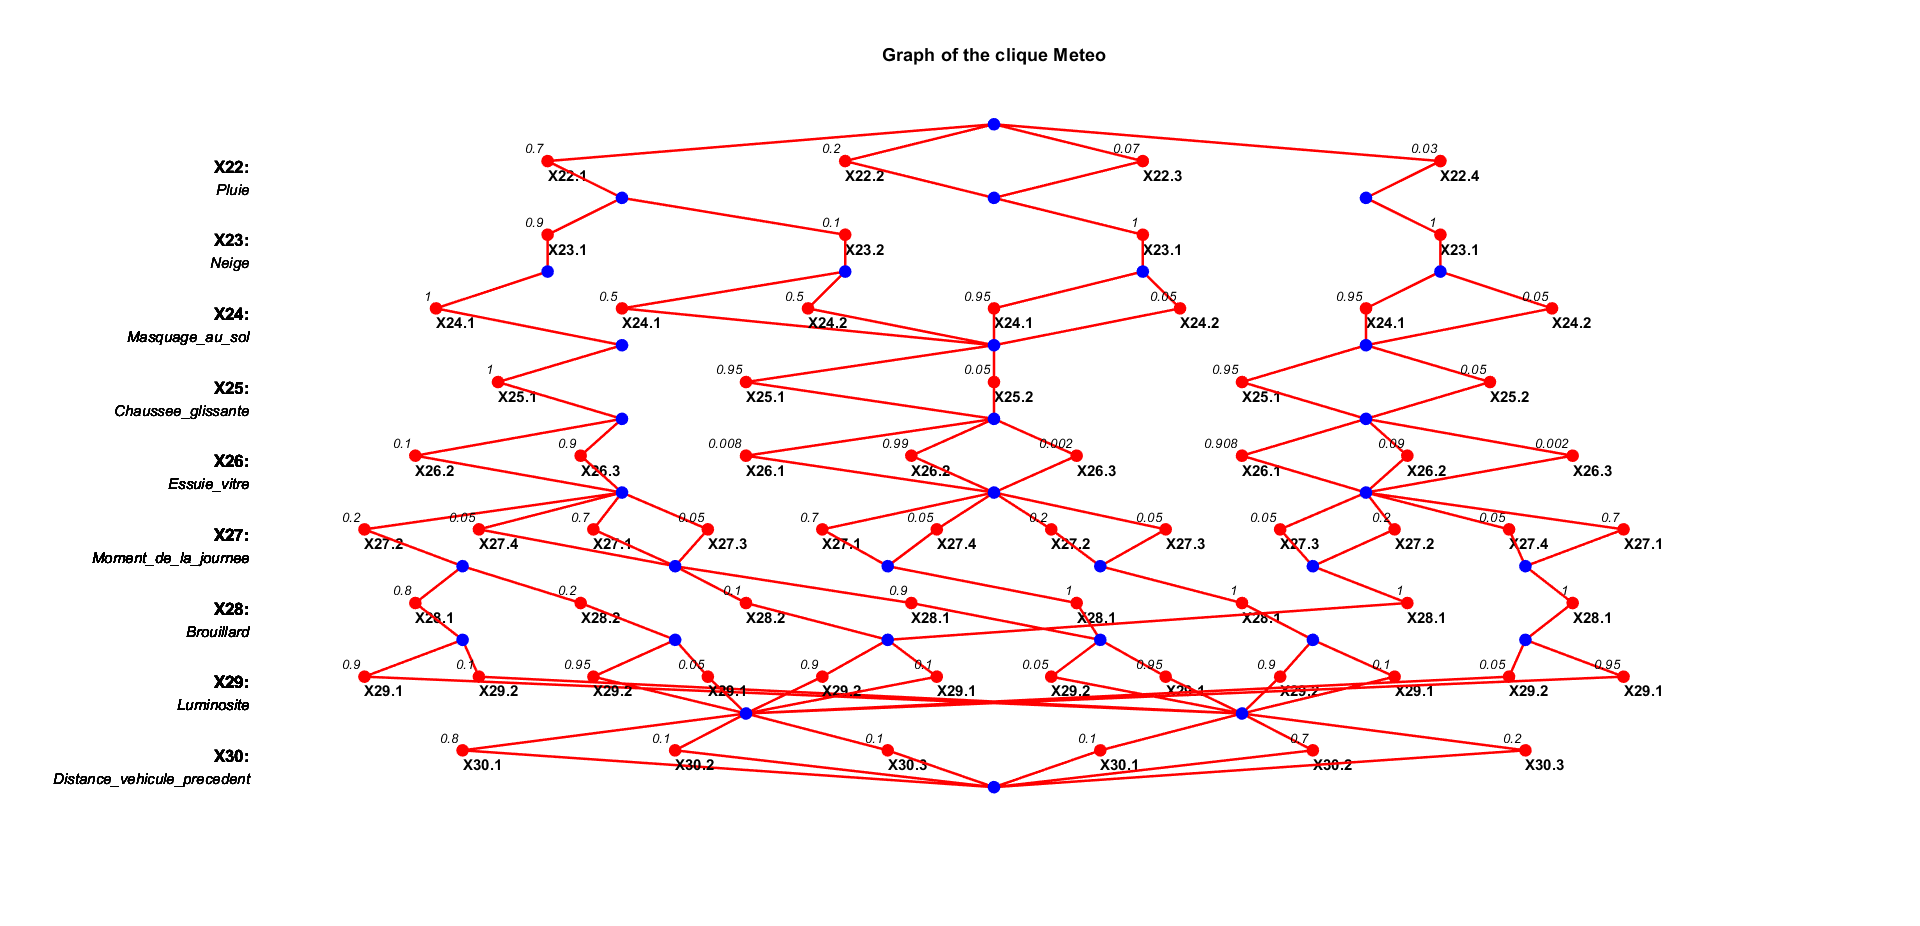
\includegraphics[width=0.8\linewidth]{../../assets/images/fig_Meteo.png}
    \caption{Phân tích dữ liệu meteorological với nhiều phương pháp kiểm định}
\end{figure}

\section{Kết luận chương}

Chương này đã trình bày chi tiết các phương pháp kiểm định thống kê quan trọng, từ những kiểm định cơ bản như Pearson chi-square và Kolmogorov-Smirnov đến các kiểm định tiên tiến hơn như Anderson-Darling và các kiểm định phi tham số. 

Những điểm chính cần ghi nhớ:
\begin{itemize}
    \item Mỗi kiểm định có điều kiện áp dụng và giả định riêng
    \item Kiểm định phi tham số mạnh mẽ hơn nhưng ít hiệu quả hơn khi giả định được thỏa mãn
    \item Cần cẩn thận với vấn đề đa so sánh và điều chỉnh mức ý nghĩa phù hợp
    \item Mô phỏng Monte Carlo là công cụ hữu ích để đánh giá và so sánh hiệu quả của các kiểm định
\end{itemize}

Các phương pháp này tạo nền tảng vững chắc cho việc phân tích dữ liệu trong thực tiễn và chuẩn bị cho các kỹ thuật phân tích nhiều chiều sẽ được trình bày trong chương tiếp theo.
